\chapter{Static dynamic bridge}
\label{chap.static_dynamic_bridge}

%\section{Coexistence between the static world and the dynamic world}
%introduction

In the programming world, there are two main families of programming language. There are the \emph{compiled}
programming, such as C, C++, Rust or Go. There are also the \emph{interpreted} programming languages, such as Python,
PHP, Lisp or Javascript. Finally, there are languages such as Java that are both at the same time.

The \emph{compiled} programming languages have the advantage of being very end-user friendly. Indeed, the implementer
distribute compiled self-sufficient binaries and the user select the binary that is compatible with his operating
system. Then, the program is supposed to work out of the box without more work than that, as illustrated
in~\cref{fig:static.dynamic.compiled.runtime}.

\begin{figure}[tbh]
  \centering
  \includegraphics[width=.6\linewidth]{figs/static_runtime}
  \caption{Compiled languages: run-time}
  \label{fig:static.dynamic.compiled.runtime}
\end{figure}

Opposite to this apparent simplicity for the end-user, all the burden is shouldered by the programmer. Indeed, to
generate a binary, there are many steps, as illustrated in~\cref{fig:static.dynamic.compiled.compiletime}. There is a
first pass with the compiler to generate intermediate machine code. Then there is a linker pass to resolve any
dependency between machine code and system code into one or multiple final distributable binaries. However, this last
pass tie the binary with a distribution. Indeed, the location of system libraries may vary between operating system,
between version of the same operating system, between compiler variants etc. Also, as the developer wants to distribute
efficient programs, he will use last optimized vectorized instructions if possible, which can tie further the binary to
a certain set of hardware supporting some assembly instructions (SSE4, XOP, FMA4, AVX-512, etc.). Upstream from those
issues, there are also issues with code. Indeed, many libraries are not cross-platform and leveraging all the
equivalences from one OS to another incurs an increase in code quantity, tests and maintenance cost to support many
platforms. For instance, the native GUI Windows libraries does not exist in Linux and must be rewritten with another
framework, such as GTK or Qt. Or else, the developer can choose to use a cross-platform GUI library from start however
this decision may not have been viable if the software was first windows-only and the cross-platform support was added
at a later date. Another caveat is that using code introspection is often very difficult at compile-time because only
few information are available (only static information). Dynamic reflection at runtime is impossible.

\begin{figure}[tbh]
  \centering
  \includegraphics[width=.6\linewidth]{figs/static_compiletime}
  \caption{Compiled languages: compile-time}
  \label{fig:static.dynamic.compiled.compiletime}
\end{figure}

The \emph{interpreted} programming language are a little less end-user friendly but are much more comfortable for
developer to distribute their software. Indeed, as shown in~\cref{fig:static.dynamic.dynamic.pipeline}, everything
happens at runtime. The maintainer only distribute the source code, the dependency list and the assets necessaries for
his program. The burden is mostly shouldered by the end-user this time. He must download and install all the language
interpreter and environment in order to execute the program from the source code. He must resolve the dependencies and
be able to execute the source code on his computer. This has the advantage of having a very rich ecosystem as
distributing, maintaining and using programs is very easy once integrated in a package manager (often delivered with the
language SDK natively). However, the main disadvantage is the performance. As the source code is not compiled into
optimized assembly code ready to be executed, the interpreter must do all the work in one go and very often this is
slow. Nowadays, all the interpreter embarks a Just-In-Time (JIT) compiler that detected the portions of a program that
are used heavily (a.k.a. hot code) and will compile them into native machine code to increase the performance
drastically without having the user pay for a long compilation time. Also, those languages usually have very developed
introspection facilities. Dynamic reflection at runtime is possible and some language, such as Common Lisp, even go
further by allowing the developer to mutate the program Abstract Syntax Tree (AST) at runtime (macro). This allows very
powerful integrations such as defining one's own DSL as if it was part of the core language itself.

\begin{figure}[tbh]
  \centering
  \includegraphics[width=.6\linewidth]{figs/dynamic_pipeline}
  \caption{Interpreted languages: run-time}
  \label{fig:static.dynamic.dynamic.pipeline}
\end{figure}

Image processing communities like to have bridges with interpretable language such as Python or Matlab, to interface
with their favorite tools, algorithms and/or facilities. As an example, with Python, the module
NumPy~\cite{oliphant.2006.numpy} is community standard which is heavily used. Henceforth, to broaden the usage of our
library, we should be able to provide a way to communicate between our library and NumPy. However, here is a showstopper:
we only distribute source code, we don't hand over binaries. Indeed, genericity in C++ is achieved via usage of template
metaprogramming. One caveat of it is that the C++ compiler cannot generate a binary until it knows which type (of image,
of value) will be used. But we don't know this information: the user (on Python's end) is not going to recompile our
library each time he has another set of types to exercise. From here, there are still multiple ways to achieve our goal.

First option is to embark a JIT (Just-in-time) compiler whose job would be to generate the binaries and bindings just as
they are used. This solution brings speed (excluding the first run that includes the compilation time) and unrestrained
genericity. However we are now bound to specificities of a compiler vendor and loose platform portability.

Another option is to type-erase our types to enables the use of various concrete types through a single generic
interface. This would translate into a class hierarchy whose concrete classes are on the leaves (thus, whose value type
and dimension are known). This induces a non-negligible slow down but allow us to keep the genericity and portability at
the cost of maintaining the class hierarchy.

Type generalization can also be considered: cast everything into a super-type that is suitable for the vast majority of
cases. For instance, we could say that we have a super-type \texttt{image4D<double>} into which we can easily cast
sub-types such as \texttt{image2D<int>} or \texttt{image3D<float>}. Of course we would loose the generic aspect and
induce non negligible speed cost. Although portability is kept.

And finally there is the dynamic dispatch. It consists in embarking dynamic information at runtime about types, and
dispatch (think of switch/case) to the correct facility which can handle those types. The obvious caveat is the cost of
maintenance induced by the genericity as we would have a number of possible dispatches that grow in a multiplicative way
with the number of handled types. Which is not very generic. On the other hand there is almost no speed loss and the
portability is guaranteed. Theoretical models exist that could bring solutions to lower the number of dispatcher to
write, such as multi-method~\cite{pirkelbauer.2010.multimethods}. Unfortunately they are currently not part of C++.

In Pylene we have chosen an hybrid solution between type-erasure and dynamic dispatch. The aim is to have a set of known
types for which we have no speed cost as well as continuing to handle other types to remain generic. To achieve this
goal, we have worked together with Célian Gossec~\cite{gossec.2019.pybind}, a student co-supervised by the authors of
this thesis, in order to provide a facility to expose our generic code to Python. As seen in the previous chapter, it is
not possible to bind C++ source code to Python. We need to have a compiled binary implementing Python binding (we chose
Pybind11~\parencite{jakob.2017.pybind11}) in order to be able to call C++ code from Python. In order to achieve the
binding without sacrificing the genericity and the performances, we have designed a solution in two steps. We do not
want to provide an abstract interface that will resolve the calls to access data on the call-site via virtual call
because it would be very slow when the C++ code is executed. This would defeat the purpose of having to rely on C++ in a
first place. However, it is possible to convert an abstract class into an instantiated concrete generic class whose
template parameter are known. This requires, however, to enumerate all the possible cases. With modern C++, it has
become possible to design $n*n$ dispatch without gigantic switch-case clauses.


\section{Hybrid solution's first step: type-erasure}

The first step of our solution consists in designing a buffer class that holds all the informations about an image:
dimension, underlying type, strides and pointer to data buffer. This class is named \texttt{ndimage\_buffer}. When
interfacing with Python, it is necessary to convert the Python image which is a \texttt{NumpPy.array} into our image
type. The purpose of this buffer image is to holds all the information from the \texttt{NumpPy.array} to then
instantiate a concrete C++ type. The first pitfall here is due to a limitation from the abstraction interface used in
Python. Indeed, when using for instance \emph{Scikit-Image}, it is not possible to differentiate a 2D multichannel image
from a 3D grayscale image. Indeed, the image is always broken down to its most simple value and a 3D multichannel image
is turned into a 3-dimensional \texttt{NumpPy.array} containing 8-bits values, the last dimension contains only 3
elements at max but can theoretically contain more as there is no limitation from the used abstraction to prevent that.
A 3D grayscale image will be broken down into a 3-dimensional \texttt{NumpPy.array} containing 8-bits values, the last
dimension will contain many values as it is expected of a 3D-image. To prevent this confusion, there is a need to
explicitly say to the Python/C++ wrapper wether the image is multichannel or not. This information must be carried
through the \texttt{ndimage\_buffer} into C++ for a correct instanciation. This process is illustrated
in~\cref{fig:type-erased.buffer}.

\begin{figure}[tbh]
  \centering
  \includegraphics[width=.6\linewidth]{figs/type-erased_buffer}
  \caption{Bridge from Python to C++ via Pybind11 and a type-erased C++ class.}
  \label{fig:type-erased.buffer}
\end{figure}

From the point of view of a practitioner, the code on the call-site (python side) should be as follow:
\begin{minted}{python}
  from skimage import data
  import numpy as np
  import Pylena as pln # our python binding
  img = data.astronaut() # 2D-rgb8 image -> Numpy.array(ndim=3, dtype='uint8')
  pln_img = pln.ndimage(img, multichannel=True) # manualy point out multichannel information
  # use(pln_img) for any pln.<algorithm> exposed to Python
\end{minted}

From the point of view of the library implementer, the code to expose the binding looks like this one:
\begin{minted}{C++}
  #include "ndimage.hpp"
  #include <pybind11/pybind11.h>

  // Expose pybind module
  void init_class_ndimage(pybind11::module& m);
  PYBIND11_MODULE(Pylena, m) { init_class_ndimage(m); }

  // declare the conversion function
  namespace mln::py {
    mln::ndbuffer_image   ndimage_from_buffer(pybind11::buffer b, bool is_multichannel = false);
    pybind11::buffer_info ndimage_to_buffer(const mln::ndbuffer_image& img);
  }

  // expose the python ndimage class with the conversion from/to py::buffer (numpy.array buffer)
  void init_class_ndimage(py::module& m) {
    using namespace pybind11::literals;

    py::class_<mln::ndbuffer_image>(m, "ndimage", py::buffer_protocol(), "is_multichannel"_a = false)
      .def(py::init(
          [](py::buffer b, bool is_multichannel = false) {
              return ndimage_from_buffer(b, is_multichannel); }))
      .def_buffer(ndimage_to_buffer);
  }
\end{minted}

This code declares a new module named \texttt{Pylena}. It then declares a class named \texttt{ndimage} which is a bridge
to Python's \texttt{buffer\_protocol}. This \texttt{buffer\_protocol} is an abstraction to allow the usage of NumPy's
array. Finally, the code declares that the class is convertible to and from the \texttt{buffer\_protocol} thanks to
provided callbacks. The code of those callbacks is as follow:

\begin{minted}{C++}
  // implement the conversion from Python to C++
  mln::ndbuffer_image ndimage_from_buffer(::py::buffer b, bool is_multichannel) {
    /* Request a buffer descriptor from Python */
    ::py::buffer_info info = b.request();

    std::ptrdiff_t      strides[16];
    int                 dims[16];
    int                 ndim = info.ndim - is_multichannel ? 1 : 0;
    int                 bpp  = info.itemsize;

    // convert the type information from Python to C++ (string to enum) for faster dispatch
    mln::sample_type_id st   = get_sample_type(info.format, is_multichannel);

    for (int i = 0; i < ndim; ++i) {
      dims[i]    = info.shape[ndim - 1 - i];
      strides[i] = info.strides[ndim - 1 - i];
    }

    if (strides[0] != bpp)
      throw std::runtime_error("Unsupported image stride along the last dimension.");

    // construct the type-erased image with all informations
    return mln::ndbuffer_image::from_buffer(
      reinterpret_cast<std::byte*>(info.ptr), st, ndim, dims, strides);
  }

  // implement the conversion from C++ to Python
  ::py::buffer_info ndimage_to_buffer(const mln::ndbuffer_image& img)
  {
    // return the python format of the underlying type, as well as information about multichanneling
    auto [ti, is_multichannel, channel_count, channel_stride] =
            get_sample_type_id_traits(img.sample_type());

    int ndim = img.pdim() + is_multichannel ? 1 : 0;

    std::vector<ssize_t> dims(ndim);
    std::vector<ssize_t> strides(ndim);

    for (int i = 0; i < ndim; ++i) {
      dims[i]    = img.size(ndim - 1 - i);
      strides[i] = img.byte_stride(ndim - 1 - i);
    }
    dims[ndim - 1]    = channel_count;
    strides[ndim - 1] = channel_stride;
    // construct the python buffer with all the information
    return ::py::buffer_info(img.buffer(), ti.size(),
            get_sample_type(img.sample_type(), is_multichannel), ndim, dims, strides);
  }
\end{minted}

This code forward informations about the buffer and handle the special case of multichannel images which Python treat
as 3D images.


\section{Hybrid solution's second step: multi-dispatcher (a.k.a. $n*n$ dispatch)}

The second step of our hybrid solution is to dispatch the type-erased code to efficient generic code. The naive way of
doing so would be to include a gigantic switch-case clause in each algorithm implementation and dispatch to the correct
instantiated generic algorithm from there. Aside from being a nightmare to maintain, the size of those clause can grow
several fold depending on the cardinality of the generic implementation. For instance, for a generic dilation, there are
3 axis of cardinality: the underlying type, the dimension, the structuring element shape. In the case where the library
support 5 different structuring element shape, 10 underlying types and 6 dimension for the image, the switch-case
statement will have 300 clauses to dispatch. And each algorithm will have to dispatch. This solution is not viable,
defeat the purpose of genericity which is to write less code in the first place. We had to find a solution to have those
dispatch while keeping our code short and efficient. The idea we took to solve this problem comes from the design of a
C++ feature, the variant, and especially the visitor. We need to have a way to write the implementation of the algorithm
once while enumerating all the possible cases. Also, if possible, the list of supported types should be written once at
one place for maintenance purpose.

We then had the idea of writing a dispatcher. This dispatcher list all the supported types and call the given callbacks
forwarding the given arguments by instantiating a specific type. For instance, let us first expose the binary threshold
operator to Python. The Python call-site code will look like this:

\begin{minted}{python}
  img_grayscale = skimage.data.grass()
  pln.operators.binary_threshold(img_grayscale)
\end{minted}

On C++ side, we need to expose the function with this code:
\begin{minted}{C++}
  void init_module_operators(pybind11::module& m);

  mln::ndbuffer_image binary_threshold(::py::buffer buffer)

  void init_module_operators(::py::module& m) {
    using namespace pybind11::literals;

    m.def("binary_threshold", binary_threshold,
          "Perform a binary threshold.\n",
          "Input"_a);
  }

  PYBIND11_MODULE(Pylena, m) {
    /* ... */

    auto operators = m.def_submodule("operators", "Image processing operators.");
    init_module_operators(operators);
  }
\end{minted}

Now that our python submodule and that our \texttt{binary\_threshold} operator are declared, let us have a look to the
operator's implementation:

\begin{minted}{C++}
  mln::ndbuffer_image dilate(::py::buffer buffer)
  {
    // grayscale image mandatory
    auto input = mln::py::ndimage_from_buffer(buffer);

    // dispatch along dimension (dimension is a valued template parameter, hence _v)
    return dispatch_v<binary_threshold_operator_t>(input.pdim(), input);
  }
\end{minted}

We have replaced the gigantic switch-case clause by a dispatcher templated by an operator. This operator will cast the
input image into the concrete generic type and call the fast generic algorithm on it. Let us have a look to what this
operator look like:

\begin{minted}{C++}
  // Operator templated by the dimension
  template <auto Dim>
  struct binary_threshold_operator_t {
    // Function templated by the image type
    template <typename Img>
    mln::ndbuffer_image operator()(Img&& img) const {
      // Cast to a grayscale (information known) of the correct dimension
      if (auto* image_ptr = std::forward<Img>(img).template cast_to<std::uint8_t, Dim>(); image_ptr)
        // call generic algorithm
        return mln::operators::binary_threshold(*image_ptr);
      else {
        std::runtime_error("Unable to convert the image to the required type.");
        return {};
      }
    }
  };
\end{minted}

This operator will attempt to cast the given image into a grayscale image of the correct dimension and then use the
resulting concrete type to pass it the fast generic \texttt{binary\_threshold} operator. Now let us have a look at where
the magic happen, at the dispatcher which list all the supported type.

\begin{minted}{C++}
template <template <auto> class V, typename... Args>
auto dispatch_v(std::size_t dim, Args&&... args) {
  switch (pdim) {
  case (1):
    return F<1>{}(std::forward<Args>(args)...);
  case (2):
    return F<2>{}(std::forward<Args>(args)...);
  case (3):
    return F<3>{}(std::forward<Args>(args)...);
  case (4):
    return F<4>{}(std::forward<Args>(args)...);
  case (5):
    return F<5>{}(std::forward<Args>(args)...);

  /* ... */

  case (0):
    [[fallthrough]];
  default:
    throw std::runtime_error("Unsupported dimension.");
}
\end{minted}

The dispatcher is instantiate the given type by the correct dimension number and then call the operator parenthesis
(function call) forwarding all the given parameters. In our case, it will instantiate the type
\texttt{binary\_threshold\_operator\_t<2>} and then call the function
\texttt{binary\_threshold\_operator\_t<2>.operator()(input)}, forwarding the input image to the underlying algorithm.

The main advantage of this approach is that all the supported features are to be listed only in one place, the
dispatcher, while any number of dispatcher can be piped to achieve the cardinality wanted. Let us push our example to
implement the mathematical morphology operator dilation. We now have two more generic axis to cover: the structuring
element shape and the underlying datatype. First, let us expose the operator to the Python code. Here is what the Python call-site look like:

\begin{minted}{python}
img_grayscale = skimage.data.grass()
rect = pln.se.rect2d(width=3, height=3)
pln.operators.dilate(img_grayscale, se)
\end{minted}

We need to expose the new structuring element's sub-module for usage in the dilation operator:

\begin{minted}{C++}
void init_module_se(pybind11::module& m);

void init_module_se(::py::module& m) {
  ::py::class_<mln::se::disc>(m, "disc").def(
      ::py::init([](float radius) { return mln::se::disc{radius}; }));

  ::py::class_<mln::se::sphere>(m, "sphere").def(::py::init([](float radius) {
    return mln::se::sphere{radius};
  }));

  ::py::class_<mln::se::rect2d>(m, "rect2d").def(::py::init([](int width, int height) {
    return mln::se::rect2d{width, height};
  }));

  ::py::class_<mln::se::rect3d>(m, "rect3d").def(::py::init([](int width, int height, int depth) {
    return mln::se::rect3d{width, height, depth};
  }));
}

PYBIND11_MODULE(Pylena, m) {
  /* ... */

  auto mse = m.def_submodule("se", "Structuring elements module.");
  init_module_se(mse);
}
\end{minted}

Now we need to expose the dilate function into the operator submodule:
\begin{minted}{C++}
// using std::variant
using se_t = std::variant<mln::se::disc, mln::se::sphere,
                          mln::se::rect2d, mln::se::cube>;

mln::ndbuffer_image dilate(::py::buffer buffer, const se_t& se)

void init_module_operators(::py::module& m) {
  /* ... */

  m.def("dilate", dilate,
    "Perform a morphological dilation.\n"
    "\n"
    "structuring element must be valid.",
    "Input"_a, "se"_a);
}
\end{minted}

We are all set to now implement the dilation operator. First, let us have a look at the underlying operator that will be
dispatched:

\begin{minted}{C++}
template <auto Dim, typename T>
struct dilate_operator_t {
  template <typename Img, typename SE>
  mln::ndbuffer_image operator()(Img&& img, SE se) const {
    if (auto* image_ptr = std::forward<Img>(img).template cast_to<T, Dim>(); image_ptr)
      return mln::dilation(*image_ptr, se);
    else {
      std::runtime_error("Unable to convert the image to the required type.");
      return {};
    }
  }
};
\end{minted}

Here we can see that we need a double dispatch. Also, the structuring element is no longue a variant and needs to be
dispatched before instantiating this operator. Finally, there is an issue here because there are two template parameter
and our dispatcher \texttt{dispatch\_v} does only handle one. We workaround this issue by writing another intermediate
operator dispatcher \texttt{dilate\_operator\_intermediate\_t} serving as trampoline that will partially instantiate the
final operator \texttt{dilate\_operator\_t} along the dimension template parameter to feed it to the last dispatcher,
\texttt{dispatch\_t}:

\begin{minted}{C++}
template <auto Dim>
struct dilate_operator_intermediate_t {
  template <typename Img, typename SE>
  mln::ndbuffer_image operator()(Img&& img, SE&& se) const {
    // Partial instantiation
    return double_dispatch_t<dilate_operator_t, Dim>(
            input.sample_type(), std::forward<Img>(input), std::forward<SE>(se));
  }
};
\end{minted}

The final function implementation will look like this:

\begin{minted}{C++}
mln::ndbuffer_image dilate(::py::buffer buffer, const se_t& se) {
  auto input = mln::py::ndimage_from_buffer(buffer);
  // dispatch the structuring elements through using std::visit for std::variant 
  return std::visit(
      [&input](const auto& se_) {
        return dispatch_v<dilate_operator_intermediate_t>(input.pdim(), input, se_);
      }, se);
}
\end{minted}

The final piece of our puzzle would be the double dispatch function that will handle the last dispatch along the
underlying data while forwarding the first dispatch along the dimension. Here is how we implemented our double dispatch:

\begin{minted}{C++}
template <template <auto, typename> class F, auto Dim, typename... Args>
auto double_dispatch_t(mln::sample_type_id tid, Args&&... args) {
  switch (tid) {
    case (mln::sample_type_id::INT8):
      return F<Dim, std::int8_t>{}(std::forward<Args>(args)...);
    case (mln::sample_type_id::INT16):
      return F<Dim, std::int16_t>{}(std::forward<Args>(args)...);
    case (mln::sample_type_id::INT32):
      return F<Dim, std::int32_t>{}(std::forward<Args>(args)...);
    case (mln::sample_type_id::UINT8):
      return F<Dim, std::uint8_t>{}(std::forward<Args>(args)...);
    case (mln::sample_type_id::UINT16):
      return F<Dim, std::uint16_t>{}(std::forward<Args>(args)...);
    case (sample_type_id::UINT32):
      return F<Dim, std::uint32_t>{}(std::forward<Args>(args)...);
    case (mln::sample_type_id::DOUBLE):
      return F<Dim, double>{}(std::forward<Args>(args)...);

      /* ... */

    case (mln::sample_type_id::OTHER):
      [[fallthrough]];
    default:
      throw std::runtime_error("Unhandled data type");
  }
}
\end{minted}

Now we have all the pieces to build operators that are agnostic from the supported data-types. Indeed, the maintainer
has gathered all the logic about listing supported data types and dimension into variant or custom dispatcher. He just
need to maintain those to enable, by default, all exposed algorithm to support them. This hybrid solution mixes
type-erasure and modern C++ facilities to allow maximum performance. Indeed, the dispatch is done before entering
algorithms and the buffer protocol facility allows us to plug directly into the Python image without having any
unnecessary copies. The only caveat would be the code bloat incurred by all the explicit instanciation leading to
compiling a large binary. Another point not covered right now would be a way to inject Python types into C++. Indeed,
our hybrid solution only support the types provided by the library. It will instantiate all the code relative to them
and support all of the combinations. But the user may be tempted to plug a user-defined type from Python as an
underlying data-type. To allow this use-case, we introduce a new concept: the \emph{value-set}. The value-set is a
standard way manipulate the underlying values. Through type-erasure, we can either manipulate a known underlying value
with native facilities (near-zero overhead) or fallback on a virtual call that may report an error or callback
user-provided Python routine to manipulate an unknown user value.


\section{Hybrid solution's third and final step: the value-set}

The \emph{value-set} is an abstraction layer around common operations needed when implementing an image processing
algorithm such as an addition, a multiplication, a type conversion, getting the maximum etc. It can be defined in C++ as
a class template whose parameter is the manipulated type. The following code shows how to define a value-set:

\begin{minted}{C++}
template <class T = void>
struct value_set {
  template <class U>
  U cast(T&& v) const { return static_cast<U>(std::forward<T>(v)); }

  T max() const noexcept { return std::numeric_limits<T>::max(); }
  T min() const noexcept { return std::numeric_limits<T>::min(); }
  /* inf, sup, ... */

  T plus(T&& v) const noexcept { return +std::forward<T>(v); }
  T minus(T&& v) const noexcept { return -std::forward<T>(v); }

  T add(T&& l, T&& r) const noexcept { return std::forward<T>(l) + std::forward<T>(r); }
  T sub(T&& l, T&& r) const noexcept { return std::forward<T>(l) - std::forward<T>(r); }
  /* mod, pow, min, max, ... */
};
\end{minted}

We can see that the default parameter of the class template is \texttt{void}. Indeed, we are inspired by what was
implemented in the standard library for \texttt{std:less} and providing a default (void) specialization in order to
improve the usability. The following code shows how to implement this specialization:

\begin{minted}{C++}
template <>
struct value_set<void> {
  template <class U, class T>
  U cast(T&& t) const { return static_cast<U>(std::forward<T>); }

  template <class T>
  T max() const noexcept { return std::numeric_limits<T>::max();}
  template <class T>
  T min() const noexcept { return std::numeric_limits<T>::min(); }
  /* ... */

  template <class T, class U>
  auto add(T&& l, U&& r) const noexcept { return std::forward<T>(l) + std::forward<U>(r); }
  template <class T, class U>
  auto sub(T&& l, U&& r) const noexcept { return std::forward<T>(l) - std::forward<U>(r); }
  /* ... */
};
\end{minted}

The template parameter is shifted from the class to the member functions. It is also important to note that the member
function are not static, which requires to instantiate the \texttt{value-set} before using it. It may sound like a
disadvantage at first glance but it can be turned into an advantage later on. Indeed, this design allows a subclass to
hold member variables which will be crucial.

Now that we have designed how our value-set is intended to work, we can deduce that an image is able to provide its own
value-set. Indeed, an image knows what values it holds and thus is able to instantiate the proper value-set
corresponding to this type. The member function returning the value-set in the class template ndimage<T, D> is then
implemented as follow:

\begin{minted}{C++}
template <class T, std::size_t D>
class ndimage {
  /* ... */
  auto get_value_set() const noexcept {
    return value_set<T>{};
  }
};
\end{minted}

For the sake of example, we are going to implement the linear stretch algorithm in order to augment the contrast. First
this algorithm construct an histogram to get both actual minimum and maximum value in the image. Then the algorithm get
the maximum and minimum values possible in the space, construct a ratio from these informations and then apply this
ratio to the image. For the sake of simplicity, we restrict our example to mono channel image. Here is how it can be
naively implemented:

\begin{minted}[linenos,highlightlines={4,9-11,14}]{C++}
  template <class T = float, class V, std::size_t D>
  mln::ndimage<T, D> stretch(mln::ndimage<V, D> img) {
    // histogram
    auto hist = std::vector<std::size_t>{std::numeric_limits<V>::max()+1, 0};
    mln::for_each(img, [&hist](V v){ ++hist[v]; });
    
    // construct ratio
    auto [m, M] = std::minmax_element(begin(hist), end(hist));
    double min = (not std::is_floating_point_v<V>) ? static_cast<double>(std::numeric_limits<V>::min()) : 0.0;
    double max = (not std::is_floating_point_v<V>) ? static_cast<double>(std::numeric_limits<V>::max()) : 1.0;
    double ratio = (max - min) / (M - m);
  
    // construct and apply scaling functor
    auto scale_fn = [m, x, r](double v) -> V { return static_cast<V>(x + (v - m) * r); };
    return mln::transform(img, scale_fn);
  }
\end{minted}

Now, we can see line 4 that we are gathering the maximum value of the input image's space. Then, line 9 and 10, we are
gathering the maximum and minimum value of the input image's space. Finally, at lines 11 and 14, we are doing
computation mixing input image's type and resulting image's type. In order to be agnostic from the way those
computations are done, we can rewrite our algorithm using value-sets as in the following code:

\begin{minted}{C++}
template <class T = float, class V, std::size_t D>
mln::ndimage<T, D> stretch(mln::ndimage<V, D> img) {
  auto img_vs = img.get_value_set();
  aut default_vs = value_set<>{}; // void specialization

  // histogram
  auto hist = std::vector<std::size_t>{img_vs.max()+1, 0};
  mln::for_each(img, [&hist](V v){ ++hist[v]; });
  
  // construct ratio
  auto [m, M] = std::minmax_element(begin(hist), end(hist));
  double min = (not std::is_floating_point_v<V>) ?
                  img_vs.template cast<double>(img_vs.min()) : 0.0;
  double max = (not std::is_floating_point_v<V>) ?
                  img_vs.template cast<double>(img_vs.max()) : 1.0;
  // equiv to (max - min) / (M - m);
  double ratio = default_vs.div(default_vs.sub(max, min), default_vs.sub(M, m));

  // construct and apply scaling functor
  auto scale_fn = [m, x, r, default_vs](double v) -> V {
    // equiv to static_cast<V>(x + (v - m) * r)
    return default_vs.template cast<V>(default_vs.add(x, default_vs.mult(default_vs.sub(v, m), r)));
  };
  return mln::transform(img, scale_fn);
}
\end{minted}

Despite loosing a little bit of expressivity (calling explicit function such as \texttt{vs.mult(..., ...)}) we are now
completely agnostic from the underlying value-type when doing any computation. In this example we are using both the
input image's value-set to gather informations about the value space limits as well as the default value-set in order to
get the computations right. Now we are able to write an algorithm independently from its underlying type on the C++
side. This feat enables one fundamental feature: type-injection from Python. Indeed, it is now possible to provide a
value-set from Python. This feat is realized simply by specializing the base value-set class over the type
\texttt{pybind::object} which is the generic way to refer to a non-trivially-convertible Python type. This
specialization is able to call the operators on any input \texttt{pybind11::object} by using a value-set coming from
Python at the construction of the image. Here is how this value-set specialization looks like on C++ side:

\begin{minted}[linenos,highlightlines={9,13,16,21,23,29}]{C++}
template <>
struct value_set<pybind11::object> {
value_set(pybind11::object python_vs_instance)
  : vs_instance_(python_vs_instance)
{}

template <typename U>
pybind11::object cast(pybind11::object v) const {
  return static_cast<U>(vs_instance_.attr("cast")(v, get_python_type<U>()));
}

pybind11::object max() const {
  return vs_instance_.attr("max")();
}
pybind11::object min() const {
  return vs_instance_.attr("min")();
}
/* ... */

pybind11::object add(pybind11::object l, pybind11::object r) const {
  return vs_instance_.attr("add")(l, r);
}
pybind11::object sub(pybind11::object l, pybind11::object r) const {
  return vs_instance_.attr("sub")(l, r);
}
/* ... */

private:
  pybind11::object vs_instance_;
};
\end{minted}

In this code we can clearly see that line 27 we are storing our Python's value-set instance into our class. This is
possible due to the fact that our value-set abstraction is not providing static class function but member function.
Hence, it is possible to offload the work of the value-set to a member variable at lines 11, 14, 19 and 22 that will
call the Python's value-set and get the wanted result. Also, at line 7 we use multiples techniques at once to get the
correct resulting cast from a Python type. First we call a function \texttt{get\_python\_type} that will return a string
containing the python-compatible representation of the resulting type we want to cast the variable into. This function
can be implemented with the C++ facilites contained in the \texttt{typeinfo} header such as the \texttt{typeid} operator
and the \texttt{std::type\_index} helper class as in the following code:

\begin{minted}{C++}
#include <cinttypes>
#include <string>
#include <typeinfo>

template <class U>
std::string get_python_type() {
  // C++ type -> Python type
  static std::unordered_map<std::type_index, std::string> type_names {
    { std::type_index(typeid(bool{})),          "bool"  },
    { std::type_index(typeid(int8_t{})),        "int"   },
    { std::type_index(typeid(int16_t{})),       "int"   },
    { std::type_index(typeid(int32_t{})),       "int"   },
    { std::type_index(typeid(int64_t{})),       "int"   },
    { std::type_index(typeid(uint8_t{})),       "int"   },
    { std::type_index(typeid(uint16_t{})),      "int"   },
    { std::type_index(typeid(uint32_t{})),      "int"   },
    { std::type_index(typeid(uint64_t{})),      "int"   },
    { std::type_index(typeid(float{})),         "float" },
    { std::type_index(typeid(double{})),        "float" },
    { std::type_index(typeid((char*){})),       "str"   },
    { std::type_index(typeid((const char*){})), "str"   },
    { std::type_index(typeid(std::string{})),   "str"   }
  };
  return type_names[std::type_index(typeid(U{}))];
}
\end{minted}

This code perform the conversion between the type information extracted from \texttt{U} with \texttt{typeid} which is
compiler specific and the corresponding Python type in order to very easily perform the type-cast on the Python side.

On this particular matter, the user will find a Python abstract class to implement in order for his value-set to be
usable by the library. This abstract class is defined by the following Python code:

\begin{minted}{python}
from abc import ABC, abstractmethod
from typing import Any
import math, importlib

class AbstractValueSet(ABC):

  @abstractmethod
  def cast(self, value: Any, type_): pass
    if type_ in ["int", "float", "bool", "str"]:
      module = importlib.import_module('builtins')
      cls = getattr(module, type_)
      return cls(value)
    else:
      raise ValueError()

  @abstractmethod
  def max(self): return math.inf

  @abstractmethod
  def min(self): return -math.inf

  # ...

  @abstractmethod
  def add(self, lhs: Any, rhs: Any) -> Any: return lhs + rhs

  @abstractmethod
  def sub(self, lhs: Any, rhs: Any) -> Any: return lhs - rhs

  # ...
\end{minted}

This abstract class provide a facility to cast a value into a given type from its representation as a string. It also
provides default / standard way of computing values. Those methods needs to be overridden by a child class as they are
all tagged with the \texttt{@abstractmethod} attribute.

Now, let us make our own custom Python data structure containing a value. Let us name our class \texttt{MyStruct} as in
the following code:

\begin{minted}{Python}
from typing import Any
class MyStruct:
  v_: Any
  def __init__(self, v: Any): self.v_ = v
  def getV(self) -> Any:      return self.v_
  def setV(self, v: Any):     self.v_ = v
\end{minted}

Now we want to use this custom structure in an image we pass to the C++ library. The following Python code will not
work:

\begin{minted}{Python}
img = np.array(
  [MyStruct(1), MyStruct(2), MyStruct(6.5), MyStruct(3.14)],
  ndmin=1)
pln_img = pln.ndimage(img, is_multichannel=false)
\end{minted}

Indeed, the image's value-type is a \texttt{pybind11::object} which requires the C++ code to fallback on the
corresponding value-set specialization. However, in order to construct a value-set of that specialization, we are
missing a parameter: the \texttt{pybind11::object} value-set offloading the work to Python. The next step is then to
declare our custom value-set on Python side shown on the following code:

\begin{minted}{Python}
from typing import Any

class MyValueSet(AbstractValueSet):
  def get_MyStruct_val__(self, v: Any):
    return v.getV() if isinstance(v, MyStruct) else v

  def cast(self, value: Any, type_):
    return super().cast(self.get_MyStruct__(value), type_)

  def max(self): return super().max()

  def min(self): return super().min()

  def add(self, lhs: Any, rhs: Any) -> Any:
    return MyStruct(super().add(self.get_MyStruct__(lhs), self.get_MyStruct__(rhs)))

  def sub(self, lhs: Any, rhs: Any) -> Any:
    return MyStruct(super().sub(self.get_MyStruct__(lhs), self.get_MyStruct__(rhs)))
\end{minted}

Now it is possible to write the following code:
\begin{minted}{Python}
  img = np.array(
    [MyStruct(1), MyStruct(2), MyStruct(6.5), MyStruct(3.14)],
    ndmin=1)
  pln_img = pln.ndimage(img, is_multichannel=false, value_set=MyValueSet())
\end{minted}

And on the C++ side there are just small trivial adaptations to do to forward the \texttt{pybind11::object} to the
\texttt{ndimage\_from\_buffer} function so that it is then correctly forwarded into the resulting
\texttt{mln::ndbuffer\_image}, thus accessible from any algorithms. There is another way of achieving the exact same
result which consist of having a concrete value-set Python class inheriting an abstract value-set C++ class. This is
rendered possible by using a trampoline on the C++ side to define a special C++ class (with macros provided by pybind).
Afterwards, it is possible to define a Python class in Python code inheriting from the trampoline intermediate C++
class. Then the user implement the pure virtual member function with Python code. Thanks to polymorphism, it is then
possible to pass this child class back to a C++ function as if it was the C++ parent class. Whichever solution is
selected, the performances remain equally bad as Python code do the work in both case.

Indeed, While it works and enables the user to construct \texttt{NumPy.array} of custom Python type and pass them to the
library with the corresponding value-set for it to "just work", the performance is greatly impacted. As a matter of
fact, the computation is no longer done on the C++ side with optimized, vectorized instructions. Instead, a callback to
Python is done in order to get the result. It is important that the user keep in mind that custom python types are be
supported by the library by providing a value-set at the cost that the resulting performances will literally be blown
away. This may be sufficient for prototyping and tinkering however the user must consider implementing his own type on
the C++ side when time comes to write production code.

\section{Performances \& overhead}

Performance-wise, the hybrid solution aims at being very competitive when comparing to the other "standard" libraries.
We want to compare to \emph{OpenCV} but also \emph{scikit-image} which are both widely use in image processing. For our
benchmark, we are simply calling a dilation on a sample image whose data are randomized but kept identical for all the
libraries. In order to conduct this benchmark, we use the Python \emph{timeit} module to evaluate the calls. Here is the
code which generate the randomized image for the benchmarks:
\begin{minted}{python}
import numpy as np
import random as rnd

def setup_test_img():
  sizes = {"width": 3138, "height": 3138}  # 10Mo
  number = 100
  percent = 20
  ref = np.zeros((sizes["width"], sizes["height"]), dtype="uint8")
  rnd.seed(42)
  for x in range(0, sizes["width"]):
    for y in range(0, sizes["height"]):
      ref[x, y] = rnd.randint(0, 255)
  return ref
\end{minted}

Now that our base image is setup, let us what we are going to mesure. We want to first compare the dilation algorithm
relative to the radius of the structuring element (disc or rectangle), as well as distinguish the shapes.

For OpenCV, the benchmarked functions will be as follow:
\begin{minted}{python}
import cv2

def bench_cv2_disc(ref, radius):
  disc = cv2.getStructuringElement(
    cv2.MORPH_ELLIPSE, (radius*2+1, radius*2+1))
  cv2.dilate(ref, disc, iterations=1)

def bench_cv2_rect(ref, width, height):
  disc = cv2.getStructuringElement(
    cv2.MORPH_RECT, (rect_width, rect_height))
  cv2.dilate(ref, disc, iterations=1)
\end{minted}

Now, for scikit-image, the benchmarked functions will be as follow:
\begin{minted}{python}
import skimage.morphology as skimorph

def bench_sckimage_disc(ref, radius):
  disc = skimorph.disk(radius, dtype="uint8")
  skimorph.dilation(ref, disc)

def bench_sckimage_rect(ref, width, height):
  rect = skimorph.rectangle(width, height, dtype="uint8")
  skimorph.dilation(ref, rect)
\end{minted}

And finally, for Pylena, we will use benchmark the following code:
\begin{minted}{python}
import Pylena as pln

def bench_pylena_rect(ref, width, height):
  rect = pln.se.rect2d(width, height)
  pln.morpho.dilate(ref, rect)

def bench_pylena_disc(ref, radius):
  disc = pln.se.disc(float(radius))
  pln.morpho.dilate(ref, disc)
\end{minted}

The resulting performance are shown in~\cref{fig:bench_python_restults}. We can see notably that for tiny structuring
elements (small radius), OpenCV is very fast thanks to hand-made optimization in the core code. Scikit-image which rely
on NumPy and then SciPy is consistently slower than both Pylena and OpenCV. It also remains stable only for a rectangle
structuring element. For a disc, the execution time grows alongside the radius of the disc. OpenCV does not remain
stable the larger the structuring element is, both for a rectangle and a disc. This may be due to the incremental nature
of the decomposition of the structuring element algorithm which decompose it in smaller 3x3 structuring elements.
However, OpenCV remains faster than Scikit-image. This algorithm remain slow for large structuring elements. Finally,
Pylena is very stable both for a rectangle and a disc. It also is consistently faster than Scikit-image image in both
cases. Compared to OpenCV, it may be slower for very small structuring elements in the case of a disc but only gets
faster than OpenCV for medium sized rectangle shaped structuring elements. We conclude that the strict decomposition
algorithm performed by Pylena allows the user to have very stable performances accross the mathematical morphology
algorithms.

\begin{figure}[tbh]
  \centering
  \begin{tabular}{cccc}
    Rectangle                                                                                          & Disc \\[5pt]
    \fbox{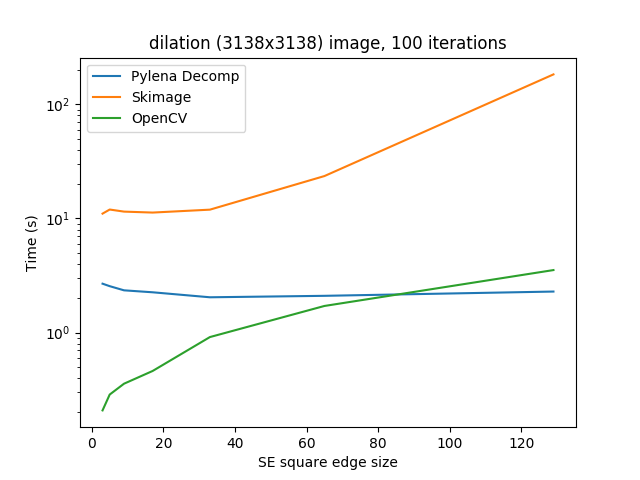
\includegraphics[width=.45\linewidth]{figs/Dilation_SERect_Benchmarks__Time_vs_SE_size.png}} &
    \fbox{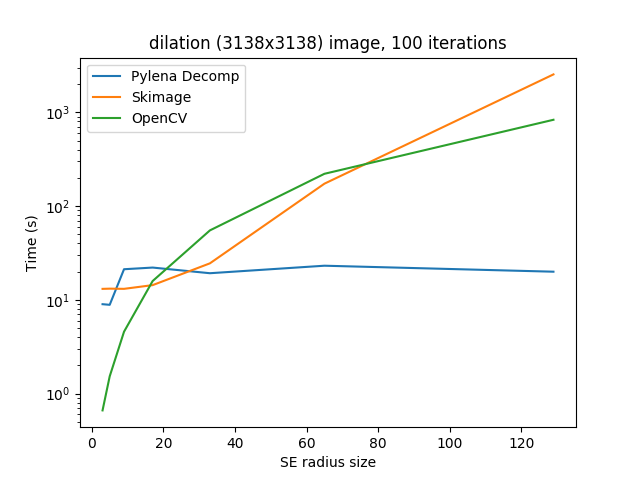
\includegraphics[width=.45\linewidth]{figs/Dilation_SEDisc_Benchmarks__Time_vs_SE_size.png}}        \\[5pt]
  \end{tabular}

  \caption{Benchmark results: OpenCV vs. Scikit-image vs. Pylena (in a dilation).}
  \label{fig:bench_python_restults}
\end{figure}

Indeed, the~\cref{fig:bench_python_restults_pln} shows the performance difference with the Pylena library when this one
does not the decomposability of its structuring elements. The algorithm using a non-decomposable structuring element has
its performances heavily impacted. Also, the algorithm is no longer stable and grows slower and slower with the radius
of the structuring elements.

\begin{figure}[tbh]
  \centering
  \begin{tabular}{cccc}
    Rectangle                                                                                             & Disc \\[5pt]
    \fbox{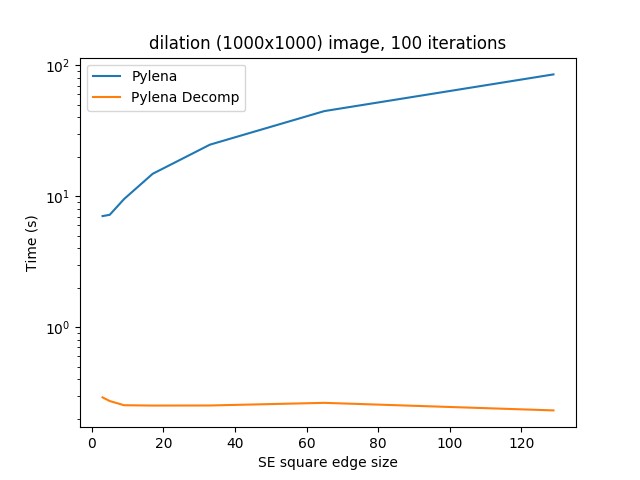
\includegraphics[width=.45\linewidth]{figs/DilationPln_SERect_Benchmarks__Time_vs_SE_size.png}} &
    \fbox{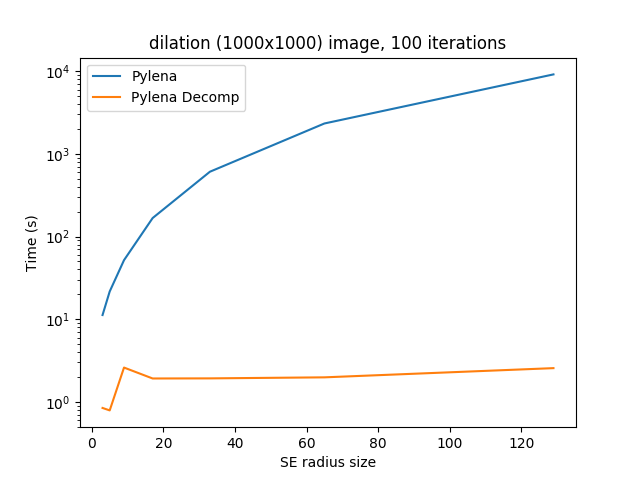
\includegraphics[width=.45\linewidth]{figs/DilationPln_SEDisc_Benchmarks__Time_vs_SE_size.png}}        \\[5pt]
  \end{tabular}

  \caption{Benchmark results: Pylena structuring elements decomposable vs. non-decomposable (in a dilation).}
  \label{fig:bench_python_restults_pln}
\end{figure}

% TODO : bench with value_set callbacks to python

\section{JIT-based solutions: pros. and cons.}

Our hybrid solution certainly has advantages but the huge disadvantage is the slowness of injecting our own types from
the Python side. There exists another solution that this thesis did not have the opportunity to study in-depth. This
solution is based on a known technology: the Just-In-Time (JIT) compilation which has been previously illustrated
in~\cref{fig:static.dynamic.dynamic.pipeline}. Indeed, it is a technology already used by interpreted languages such as
Java or PHP to generate on-the-fly native and optimized machine code for the section of the source code that is
considered "hot" by the interpreter. A source code is "hot" when it is executed a lot: the end-user would gain paying
the compilation time once to have this code executed faster several times later on. When applying this strategy to our
problematic, it would mean that the user must be able to compile native machine code from the templated generic C++ code
by injected the requested type when it is used. Such an operation shift heavily the burden on the user and it is
well-known that compiling C++ code is notably \emph{complicated} and \emph{slow}. In addition, the library needs to be
able to auto-generate python-binding once the code is compiled. There are several solutions to achieve this process.

The first solution is to basically use system call to the compilers to actually \emph{compile} C++ code once the
templated types are known and explicitly instanciated in the source code. This solution requires careful code-generation
design and that the user actually possess a compiler on his computer. Furtheremore, the user must resolve all the
library dependencies, such as \emph{freeimage} for IO etc. This solution was engineered in the
library~\parencite{demaille.2013.vcsn}. Indeed, each time the user declared a new automata in his jupyter notebook,
corresponding source code is compiled in the foreground and then cached. It is a very perilous solution to implement
when the final execution environment (OS, installed software) is not well-known in advance. Nowadays, the issue may be
lesser, however, it still requires to maintain both the library and the container solution to use it.

The second solution is to use Cython~\parencite{behnel.2010.cython}. It is a transpiling infrastructure which transform
a Python source code directly into C-language source code so that it can be compiled by a standard C compiler just by
linking against the Python/C API. This remove the burden of writting the careful code-generation routine, system-calls
to the C++ compiler and removes the need to resolve all the dependencies. This infrastructure takes care of everything
for the user. Also, by transpiling it into C code, it is faster because a C compiler is faster than a C++ compiler. The
big issue here is that C code has no support for templates. This means that instead of having to compile instanciated
C++ templated code directly, we need to write some glue code to call templated C++ code from the generated C code from
Python. Sadly the main issue here is not solved, just shifted.

The third solution consists in relying on recent projects that are all relying on the LLVM infrastructure. We can
notably note Autowig~\parencite{fernique.2018.autowig}, Cppyy~\parencite{wimtlplavrijsen.2016.cppyy} and
Xeus-cling~\parencite{quantstack.2021.xeus-cling}. Autowig has in-house code based on LLVM/Clang to parse C++ code in
order to generate and compile a Swig Python binding using the Mako templating engine. Autowig, coupled with Cython would
permit the user to, for instance, generate C code related to a custom Python structure. Then a simple call to Autowig
will parse the C code and inject it into the C++ library to generate the appropriate bindings for the user. As for
Cppyy, it is based on LLVM/Cling, a C++ interpreter, and can directly interpret C++ code from a python string. This
allow for easy injection of custom types, be they in Python code (transpiled with Cython) or C++ code (directly
interpreted by Cling). Afterwards, the infrastructure generates the appropriate binding from the templated C++ library
for the injected type. Finally, Xeus-cling is a ready-to-use jupyter kernel and allow the usage of C++ code directly
from within a notebook. This completely bypass the need of a Python binding in the first place and allow the user to use
the library from within the notebook as if he was using a Python library. However all those infrastructure come with a
hefty cost in term of binary size. Indeed, a C++ compiler is not small and embarking it alongside the image processing
library can easily impact greatly the final binary. Without the LLVM infrastructure the binary may weight around 3MB.
With the LLVM infrastructure, the binary weight at the bare minimum 50MB. Also, these solutions may not be immediately
faster. Indeed, when prototyping back and forth with a variety of types, the user may not be eager to wait for long
compilations times each time he is testing with a an iteration of his work. Despite those facts, those solutions offers
great avenue of research for the future and the author is eager to thread those paths.
